\documentclass{article}

% compile with
%
%  pdflatex -shell-escape potfit_logo

\usepackage[utf8]{inputenx}
\usepackage[T1]{fontenc}
\usepackage{tikz}
\usepackage{gnuplot-lua-tikz}
\usetikzlibrary{shapes,arrows,backgrounds,positioning,fit,calc,
  decorations.pathreplacing,decorations.pathmorphing,fadings,decorations.markings,
  intersections,shadows}

\usepackage{fouriernc}

\begin{document}

  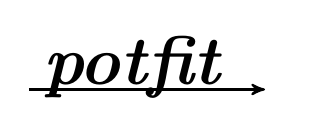
\begin{tikzpicture}
    \draw[->, thick, >=stealth'] (1.8,0) -- (4.8,0) node[anchor=west] {};
    \draw[samples=80,domain=1.93:4.6, red, very thick] plot
      function{4*0.8*((2/x)**12-(2/x)**6)+0.02};
    \node[] at (3.15,0.279) {\Huge\textit{\textbf{potfit}}};
  \end{tikzpicture}%

\end{document}
